
\begin{filecontents*}{document.bib}
@article{forexTrend2011,
	title   = {FOREX Trend Classification using Machine Learning Techniques},
	year    = {2011}
}
@article{deepTechnicalAnalysis2021,
	title   = {Can Deep Learning Improve Technical Analysis of Forex Data to Predict Future Price Movements?},
	year    = {2021}
}
@article{financialTradingGame2018,
	title   = {Financial Trading as a Game: A Deep Reinforcement Learning Approach},
	year    = {2018}
}
@article{macroQuant2025,
  author = {Kagadal, Darshan and Varma, Angad and {Ayush} and Desai, Bhargav},
  title = {Macro-Quant: A Hybrid Machine Learning Framework for Non-Stationary Exchange Rate Forecasting ({USD/INR})},
  journal = {International Journal of Research in Engineering \& Science},
  volume = {9},
  number = {6},
  year = {2025},
  doi = {10.5281/zenodo.17929713}
}
@article{deepLstmRl2019,
	title   = {Deep LSTM with Reinforcement Learning Layer for Financial Trend Prediction in FX High Frequency Trading Systems},
	year    = {2019}
}
@article{algoMl2022,
	title   = {An Ensembling Architecture Incorporating Machine Learning Models and Genetic Algorithm Optimization for Forex Trading},
	year    = {2022}
}
\end{filecontents*}

\documentclass[12pt,oneside,letterpaper,english]{article}

\usepackage[T1]{fontenc}
\usepackage[utf8]{inputenc}
\usepackage[margin=2.25cm,headheight=26pt,includeheadfoot]{geometry}
\usepackage[english]{babel}
\usepackage{titlesec}
\usepackage{amsmath,amssymb}
\usepackage[colorlinks=true,linkcolor=black,urlcolor=blue,citecolor=blue]{hyperref}
\usepackage{graphicx}
\usepackage{fancyhdr}
\usepackage{lastpage}
\usepackage{caption}
\usepackage{tocloft}
\usepackage{setspace}
\usepackage{booktabs}
\usepackage{array}
\usepackage{tabularx}
\usepackage{longtable}
\usepackage{lscape}
\usepackage{enumitem}
\usepackage{microtype}
\usepackage{natbib}

\graphicspath{{figures/}}
\bibliographystyle{ieeetr}

\title{Literature Review and Toy Model for Machine Learning in Forex}
\author{Prince Kumar, Roll No. -- 230051013}
\newcommand{\supervisorname}{Dr. Raghunath Sahoo\\Dr. Kalindi C. Pradhan}

\setlength{\parindent}{2em}
\makeatletter\let\Title\@title\makeatother
\renewcommand{\rmdefault}{ptm}
\renewcommand{\headrulewidth}{1pt}
\renewcommand{\footrulewidth}{1pt}
\pagestyle{fancy}
\fancyhf{}
\rhead{\nouppercase{\rightmark}}
\lhead{\Title}
\setlength{\headheight}{26pt}
\setlength{\footskip}{50pt}
\cfoot{\thepage}
\titleformat{\section}{\large\bfseries\sffamily\raggedright}{\thesection}{1em}{}
\titleformat{\subsection}{\large\bfseries\sffamily\raggedright}{\thesubsection}{1em}{}
\titleformat{\subsubsection}{\normalsize\bfseries\sffamily\raggedright}{\thesubsubsection}{1em}{}

\newcolumntype{Y}{>{\raggedright\arraybackslash}X}
\newcolumntype{L}[1]{>{\raggedright\arraybackslash}p{#1}}
\newcommand{\metric}[1]{\textit{#1}}

\begin{document}

\pagenumbering{roman}

\begin{titlepage}
\begin{center}
\vspace{2cm}
%\textsc{Oregon State University}\\[1.5cm]

\includegraphics[scale=0.1]{root/IITI_Logo.png}~\\[1cm]

{\LARGE\bf Department of Physics, IIT Indore}

\vspace{2cm}

% Title
\hrule
\vspace{.5cm}
{ \huge \bfseries Literature Review and Baseline models Report} % title of the report
\vspace{.5cm}

\hrule
\vspace{1.5cm}

\textsc{\textbf{Author}}\\
\vspace{.5cm}
\centering

% add your name and roll no. here
{\large\bf Prince Kumar (230051013)} \\

\vspace{2cm}

\textsc{\textbf{Supervisor}}\\
\vspace{.5cm}
\centering

{\large\bf \supervisorname} \\

\vspace{2cm}

\centering \today % see latexmkrc for time zone change
\end{center}
\end{titlepage}

\begin{abstract}
	This report reviews eight representative studies on machine learning and deep learning for foreign-exchange prediction and trading. The literature covers classification, technical-indicator systems, reinforcement learning, high-frequency forecasting, macroeconomic features, and ensemble methods. A small, reproducible toy model is then specified as a baseline for next-day directional prediction. The model definition, data protocol, parameters, and evaluation plan are documented here; numerical model evaluations will be added as experiments are completed.
\end{abstract}
\newpage

\addcontentsline{toc}{section}{Table of Contents}
\tableofcontents
\thispagestyle{fancy}
\newpage

\pagenumbering{arabic}
\doublespacing
\thispagestyle{fancy}

\section{Introduction}

The purpose of this report is twofold. First, it organizes a small literature review around the prediction task, input data, architecture, and evaluation protocol. Second, it defines a deliberately simple toy model that can serve as a transparent reference point for later experiments.

The current report is an interim study document. It records the model specifications and the evaluation fields that will be used for the complete model comparison. It does not claim that the toy model is production-ready or that historical performance guarantees future returns.

\section{Literature Review}

The reviewed papers show a progression from engineered technical features and conventional classifiers toward image-based deep learning, recurrent networks, reinforcement learning, and hybrid ensembles. They also illustrate an important distinction between predicting a label and earning a return. For example, Macro-Quant reports directional accuracy above a random baseline but a negative absolute trading return, while several other studies report positive returns using richer action-selection or trading-simulation layers.

\begin{landscape}
\scriptsize
\setlength{\tabcolsep}{3pt}
\renewcommand{\arraystretch}{1.25}
\begin{longtable}{@{}>{\centering\arraybackslash}p{0.45cm}L{1.6cm}L{0.45cm}L{1.75cm}L{1.4cm}L{1.4cm}L{1.6cm}L{2.0cm}L{2.1cm}L{1.6cm}L{1.5cm}L{2.1cm}@{}}
\caption{Summary of selected literature on machine learning for foreign-exchange prediction and trading.}
\label{tab:literature-review}\\
\toprule
\textbf{S.No.} & \textbf{Paper} & \textbf{Year} & \textbf{Type of Prediction} & \textbf{Currency Pair / Market} & \textbf{Timeframe} & \textbf{Data Source} & \textbf{Inputs / Features} & \textbf{Model / Architecture} & \textbf{Baseline / Comparison} & \textbf{Evaluation Metrics} & \textbf{Main Result} \\
\midrule
\endfirsthead
\multicolumn{12}{c}{\tablename\ \thetable{} -- continued from previous page} \\
\toprule
\textbf{S.No.} & \textbf{Paper} & \textbf{Year} & \textbf{Type of Prediction} & \textbf{Currency Pair / Market} & \textbf{Timeframe} & \textbf{Data Source} & \textbf{Inputs / Features} & \textbf{Model / Architecture} & \textbf{Baseline / Comparison} & \textbf{Evaluation Metrics} & \textbf{Main Result} \\
\midrule
\endhead
\midrule
\multicolumn{12}{r}{Continued on next page} \\
\endfoot
\bottomrule
\endlastfoot
1 & \textit{FOREX Trend Classification using Machine Learning Techniques} & 2011 & Binary classification: next-day High or Low & USD/JPY, USD/EGP, EUR/EGP, EUR/SAR & Daily; 1--30 day history & OHLCV, Apr 2003--Aug 2010; 1852 days & 81 features: 46 technical-analysis features, 2 GARCH features, and signal-processing features including averages, slopes, Fourier, and sine terms & SVM, MLP, and RBF; feature selection / extraction with SVM, Bagging Trees, PCA, LDA, MCML, and NCA & Feature-selection / extraction methods and classifiers & Accuracy (\%) and PNP & Best accuracy 79.8\% for EUR/SAR; best PNP 67.7\% for EUR/EGP \\
2 & \textit{Can Deep Learning Improve Technical Analysis of Forex Data to Predict Future Price Movements?} & 2021 & Trading action classification: Buy / Sell / Stay & GBP/USD, EUR/USD, USD/CHF, USD/JPY, EUR/GBP, GBP/JPY & Four-hour candles; 80 hours of context; next three candles & MetaTrader 5 historical data, 2010--2021 & Candlestick-chart images, 20 technical indicators, and trading rules & ResNet50 and Vision Transformer (ViT), combined with a Genetic Algorithm and trading simulation & Hernandez-Aguila et al., Munkhdalai et al., and Buy-and-Hold & Net Profit, Total Trades, Profit Factor, Expected Payoff, Drawdown, Recovery Factor, and Sharpe Ratio & About 20.2\% average gain and outperformed alternatives on almost all markets; the learned AI rule itself did not form an effective prediction strategy \\
3 & \textit{Financial Trading as a Game: A Deep Reinforcement Learning Approach} & 2018 & Trading decision: Long / Neutral / Short & 12 major and cross Forex pairs; no INR & 15-minute intervals & TrueFX tick data, 2012--2017 & Eight recent close log returns and tick volume for all 12 pairs; sine-transformed minute, hour, and day; current position & Financial DRQN: two linear layers, LSTM, and three-output layer, with action augmentation & Buy-and-hold, sell-and-hold, epsilon-greedy, and action augmentation & Annual return, Sharpe, Sortino, maximum drawdown, cumulative return, and win rate & Positive returns for all 12 pairs \\
4 & \textit{Macro-Quant: A Hybrid Machine Learning Framework for Non-Stationary Exchange Rate Forecasting} & 2025 & Five-day directional prediction: Up / Down & USD/INR & Daily; direction over five days & Yahoo Finance and FRED & Daily OHLC plus US--India yield spreads, inflation/CPI differential, crude oil, VIX, and trade balances & XGBoost classifier with stationarity transformation and SHAP explainability & Random Walk and Logistic Regression; the random baseline was not competitive & Accuracy, Precision, Recall, F1-score, confusion matrix, SHAP importance, Sharpe Ratio, and financial return & 60.96\% accuracy versus 58.11\% for Logistic Regression and 50\% random baseline; trading strategy produced a $-16\%$ absolute return \\
5 & \textit{Deep LSTM with Reinforcement Learning Layer for Financial Trend Prediction in FX High Frequency Trading Systems} & 2019 & Trend classification: SHORT / LONG / Trading Range & EUR/USD, with correlated EUR/GBP and GBP/USD & One-minute candles; 100 candles in, next 100 candles predicted & Tickstory historical FX data, 2004--2018 & Closing prices of EUR/USD, GBP/USD, and EUR/GBP, normalized to $[0,1]$ & Two-layer LSTM with 300 cells per layer, fully connected and SoftMax classification layers, followed by an RL Motor Map correction & LSTM-only versus LSTM plus RL correction & Classification accuracy, ROI, and maximum drawdown & LSTM alone about 70\% accuracy; RL correction about 85\% average accuracy, 98.23\% ROI, and 15.97\% maximum drawdown \\
6 & \textit{Explainable Reinforcement Learning on Financial Stock Trading using SHAP} & Not stated & Trading action / reward prediction: Buy or Sell & SENSEX and DJIA; individual stocks & Daily; 30-day sliding window & Yahoo Finance & OHLCV and the previous 30 days of trading states and actions & Deep Q-Network (DQN) with SHAP for local post hoc explanations & No explicit predictive baseline & Reward prediction, training MSE, and qualitative SHAP waterfall explanations & DQN generates Buy/Sell actions and reward predictions; SHAP identifies which past states and actions contributed most \\
7 & \textit{An Ensembling Architecture Incorporating Machine Learning Models and Genetic Algorithm Optimization for Forex Trading (AlgoML)} & 2022 & Next-day Buy/Sell signal prediction & EUR/USD & Daily; 30-day lookback for deep-learning models & Broker/OANDA data; training 2006/2010--2018, test 2020 & OHLCV and 13 technical indicators, 19 parameters; fractional differencing ($d=0.8$) and normalization & Ensemble of DQN, A2C, PPO, CNN, CNN-BiLSTM, and BiLSTM, with GA-optimized Pullback strategy and majority voting & Individual models, Prophet, SVM/RF exploration, and GA Pullback & Accuracy, Buy/Sell F1, net P\&L, and maximum drawdown & Ensemble: 9.97\% net P\&L, 0.55 accuracy, and $-0.68\%$ maximum drawdown; GA Pullback achieved best P\&L at 10.55\% \\
8 & \textit{An Automated FX Trading System Using Adaptive Reinforcement Learning} & 2006 & Trading signal / position prediction: Long vs Short & EUR/USD & 1-minute high-frequency data & HSBC Bank, London; Jan 2000--Jan 2002 & Past FX price changes/returns, current position, and experiments with 14 technical indicators & Recurrent Reinforcement Learning (RRL) with a recurrent single-layer neural network, risk-management layer, and dynamic utility optimization layer (Adaptive Reinforcement Learning) & RRL/basic system versus dynamic optimization; buy-and-hold comparison & Cumulative profit, risk factor, average profit/trade, correct-direction percentage, utility, and drawdown/risk & 5,104 pips (about 26\% p.a.) versus $-1,636$ pips (about $-8\%$ p.a.) for buy-and-hold; approximately 61--63\% correct direction; dynamic optimization consistently improved utility \\
\bottomrule
\end{longtable}
\end{landscape}

\subsection{Observations from the Literature}

Several design choices recur across the studies:
\begin{itemize}[leftmargin=1.5cm]
	\item \textbf{Task definition:} The prediction target ranges from a binary direction label to a trading action or a position-aware reinforcement-learning decision.
	\item \textbf{Feature design:} Technical indicators and lagged prices remain common, while macroeconomic variables, correlated currency pairs, time encodings, and chart images provide alternative information sources.
	\item \textbf{Evaluation:} Classification metrics alone are insufficient. Return, drawdown, Sharpe ratio, and transaction-aware simulation are needed to assess whether predictions translate into a useful strategy.
	\item \textbf{Validation risk:} Because exchange-rate data are time ordered and non-stationary, random shuffling can leak future information. Chronological splits and walk-forward testing are more appropriate for the experiments that follow.
\end{itemize}

\subsection{Research Gap: Post Hoc Analysis of Forex Reinforcement Learning}

The reviewed Forex studies use reinforcement learning to select trading actions or to correct predictions, but they do not provide a systematic post hoc explanation of the learned policy. The stock-finance study \textit{Explainable Reinforcement Learning on Financial Stock Trading using SHAP} provides a related precedent: a DQN is combined with SHAP to produce local waterfall explanations showing which earlier trading states and actions contributed to a Buy/Sell decision and its predicted reward. However, this analysis is performed for stock markets rather than foreign exchange.

This creates a focused research opportunity: apply post hoc explainability to a Forex reinforcement-learning agent and test whether explanations remain stable across currency pairs, market regimes, and action types. A suitable study could combine SHAP explanations with action validity, reward attribution, temporal stability, and trading metrics such as return, drawdown, and Sharpe ratio. The explanation should be evaluated not only visually but also for consistency under small perturbations of the input state and for agreement with the agent's action-value differences.

\section{Toy Models and Experimental Setup}

\subsection{Objective and Target}

The notebooks implement next-day point prediction for the INR series rather than binary classification. Let $C_t$ denote the INR value at day $t$. The target is
\[
    y_t = C_{t+1}.
\]
Directional accuracy is computed afterward by comparing the sign of the predicted and observed day-to-day movements. This separates the regression objective from the secondary question of whether the model predicts the market direction correctly.

\subsection{Data and Features}

The data are loaded from the FRED directory. The target column is \texttt{INR}; the base exogenous features are \texttt{JPY}, \texttt{EUR}, \texttt{FFER}, and \texttt{US10YY}. The data are prepared chronologically, with 80\% used for training, 10\% for validation, and 10\% for testing. The next-day target is created with a one-step shift, and rows without a target are removed.

The technical-indicator experiment adds 18 derived features to the four base variables and the current INR value:
\begin{itemize}[leftmargin=1.5cm]
	\item \texttt{MA\_5}, \texttt{MA\_10}, \texttt{MA\_30}, \texttt{MA\_50}, and \texttt{MA\_100};
	\item \texttt{EMA\_5}, \texttt{EMA\_10}, \texttt{EMA\_30}, \texttt{EMA\_50}, and \texttt{EMA\_100};
	\item \texttt{RSI};
	\item \texttt{BB\_Middle}, \texttt{BB\_Upper}, and \texttt{BB\_Lower};
	\item \texttt{Volatility};
	\item \texttt{ATR\_14\_proxy} and \texttt{ATR\_\%\_proxy}; and
	\item \texttt{Log\_Returns}.
\end{itemize}
Thus, the technical-indicator input contains 23 columns in total. In this branch, the target is the next log return, created as \texttt{Log\_Returns.shift(-1)}, rather than the next INR level. The feature and target scalers are fitted on the training split.

\subsection{Baseline Models}

The experiments use the following transparent baselines:
\begin{itemize}[leftmargin=1.5cm]
    \item \textbf{Naive:} predicts using the previous INR value.
    \item \textbf{Moving Average:} predicts using the moving-average baseline implemented in \texttt{utils.py}.
    \item \textbf{ARIMA:} uses the four base exogenous features, with order $(2,0,1)$ selected by grid search over $p,q\in\{0,1,2\}$ and $d\in\{0,1\}$.
    \item \textbf{XGBoost:} uses 500 estimators, learning rate 0.03, maximum depth 5, subsample 0.8, column subsample 0.8, and random state 42.
    \item \textbf{Linear Regression:} a PyTorch linear layer trained with Adam at learning rate 0.01 for 100 epochs using MSE loss.
\end{itemize}

\subsection{Neural Network Models}

All models predict a continuous next-day target and therefore use mean squared error (MSE) as the training loss.

\begin{table}[h!]
\centering
\caption{Neural-network model architectures and training configuration.}
\label{tab:neural-model-architectures}
\scriptsize
\setlength{\tabcolsep}{3pt}
\renewcommand{\arraystretch}{1.25}
\begin{tabularx}{\textwidth}{@{}L{2.05cm}Y L{3.35cm}L{1.25cm}L{1.7cm}L{1.25cm}L{1.25cm}L{1.7cm}@{}}
\toprule
\textbf{Model} & \textbf{Input} & \textbf{Architecture} & \textbf{Activation / output} & \textbf{Loss} & \textbf{Optimizer} & \textbf{Learning rate} & \textbf{Epochs / status} \\
\midrule
Base deep & 5 standardized base features & Linear(5,64) $\rightarrow$ Linear(64,32) $\rightarrow$ Linear(32,1) & ReLU / 1 value & MSE & Adam & 0.01 & 100; executed \\
Linear + technical indicators & 23 standardized features & Linear(23,1) & None / 1 value & MSE & Adam & 0.001 & 100; executed \\
Deep + technical indicators & 23 standardized features & Linear(23,64) $\rightarrow$ Linear(64,32) $\rightarrow$ Linear(32,1) & ReLU / 1 value & MSE & Adam & 0.001 & 100; executed \\
Deep + technical + temporal & Technical features with temporal-data path & Linear(\textit{d},128) $\rightarrow$ Linear(128,64) $\rightarrow$ Linear(64,1), with Dropout(0.2) & ReLU / 1 value & MSE & Adam & Configured & 100; executed \\
LSTM extension & Five-lag temporal input & Five-lag LSTM cell followed by a prediction layer & LSTM / 1 value & MSE & Not run & Not run & Future extension \\
\bottomrule
\end{tabularx}
\end{table}

Here, $d$ denotes the feature dimension produced by the temporal-data path.

\begin{table}[h!]
\centering
\caption{Experimental configuration used by the toy-model notebooks.}
\label{tab:toy-parameters}
\begin{tabular}{ll}
\toprule
\textbf{Parameter} & \textbf{Setting} \\
\midrule
Target & Next-day INR value \\
Base features & JPY, EUR, FFER, US10YY \\
Split & 80\% train, 10\% validation, 10\% test \\
Training batch size & 32 (configured) \\
Neural-network epochs & 100 \\
Base deep architecture & Linear(5,64)-ReLU-Linear(64,32)-ReLU-Linear(32,1) \\
Technical deep architecture & Linear-64-ReLU-32-ReLU-1 \\
Temporal deep architecture & Linear-128-ReLU-Dropout(0.2)-64-ReLU-Dropout(0.2)-1 \\
Loss & Mean squared error \\
Optimizers & Adam; learning rate 0.01 or 0.001 by experiment \\
\bottomrule
\end{tabular}
\end{table}

\section{Evaluation Report}

The evaluation notebook recomputes regression and directional metrics against the currently loaded target splits. The results below are therefore taken from the latest notebook evaluation rather than the earlier values stored in the model-results artifact.

\begin{table}[h!]
\centering
\caption{Latest evaluation results from the evaluation notebook.}
\label{tab:toy-results}
\scriptsize
\setlength{\tabcolsep}{4pt}
\begin{tabular}{llrrrrr}
\toprule
\textbf{Model} & \textbf{Split} & \textbf{MAE} & \textbf{MSE} & \textbf{RMSE} & \textbf{MAPE (\%)} & \textbf{Direction (\%)} \\
\midrule
Moving Average & Train & 0.1813 & 0.1232 & 0.3510 & 0.33 & 55.35 \\
Naive & Train & 0.2082 & 0.1293 & 0.3596 & 0.38 & 54.83 \\
Linear + Technical Indicators & Train & 0.6548 & 0.9749 & 0.9874 & 1.22 & 59.29 \\
Deep + Technical Indicators & Train & 0.6690 & 1.0007 & 1.0003 & 1.24 & 59.09 \\
Deep + Technical + Temporal & Train & 0.6708 & 1.0098 & 1.0049 & 1.25 & 58.86 \\
Deep + Technical Indicators & Test & 0.2220 & 0.1090 & 0.3302 & 0.25 & 53.53 \\
Deep + Technical + Temporal & Test & 0.2319 & 0.1080 & 0.3286 & 0.26 & 55.85 \\
Linear + Technical Indicators & Test & 0.3186 & 0.1659 & 0.4074 & 0.36 & 46.47 \\
\bottomrule
\end{tabular}
\end{table}

The latest test results show that the deep model with technical indicators has the lowest MAE (0.2220), while the temporal-feature model has the highest directional accuracy (55.85\%) and the lowest test MSE (0.1080). The linear technical-indicator model has the weakest test directional accuracy at 46.47\%. The train--test gap in directional accuracy also shows why the test split, rather than training performance, should drive model selection.

Figures~\ref{fig:evaluation-regression-test}--\ref{fig:evaluation-predictions-test} reproduce representative plots generated by evaluate.ipynb. The regression comparison highlights the error scale across models, the directional plot compares train and test behavior, and the prediction plot shows how each model tracks the held-out target series.

\begin{figure}[htbp]
\centering
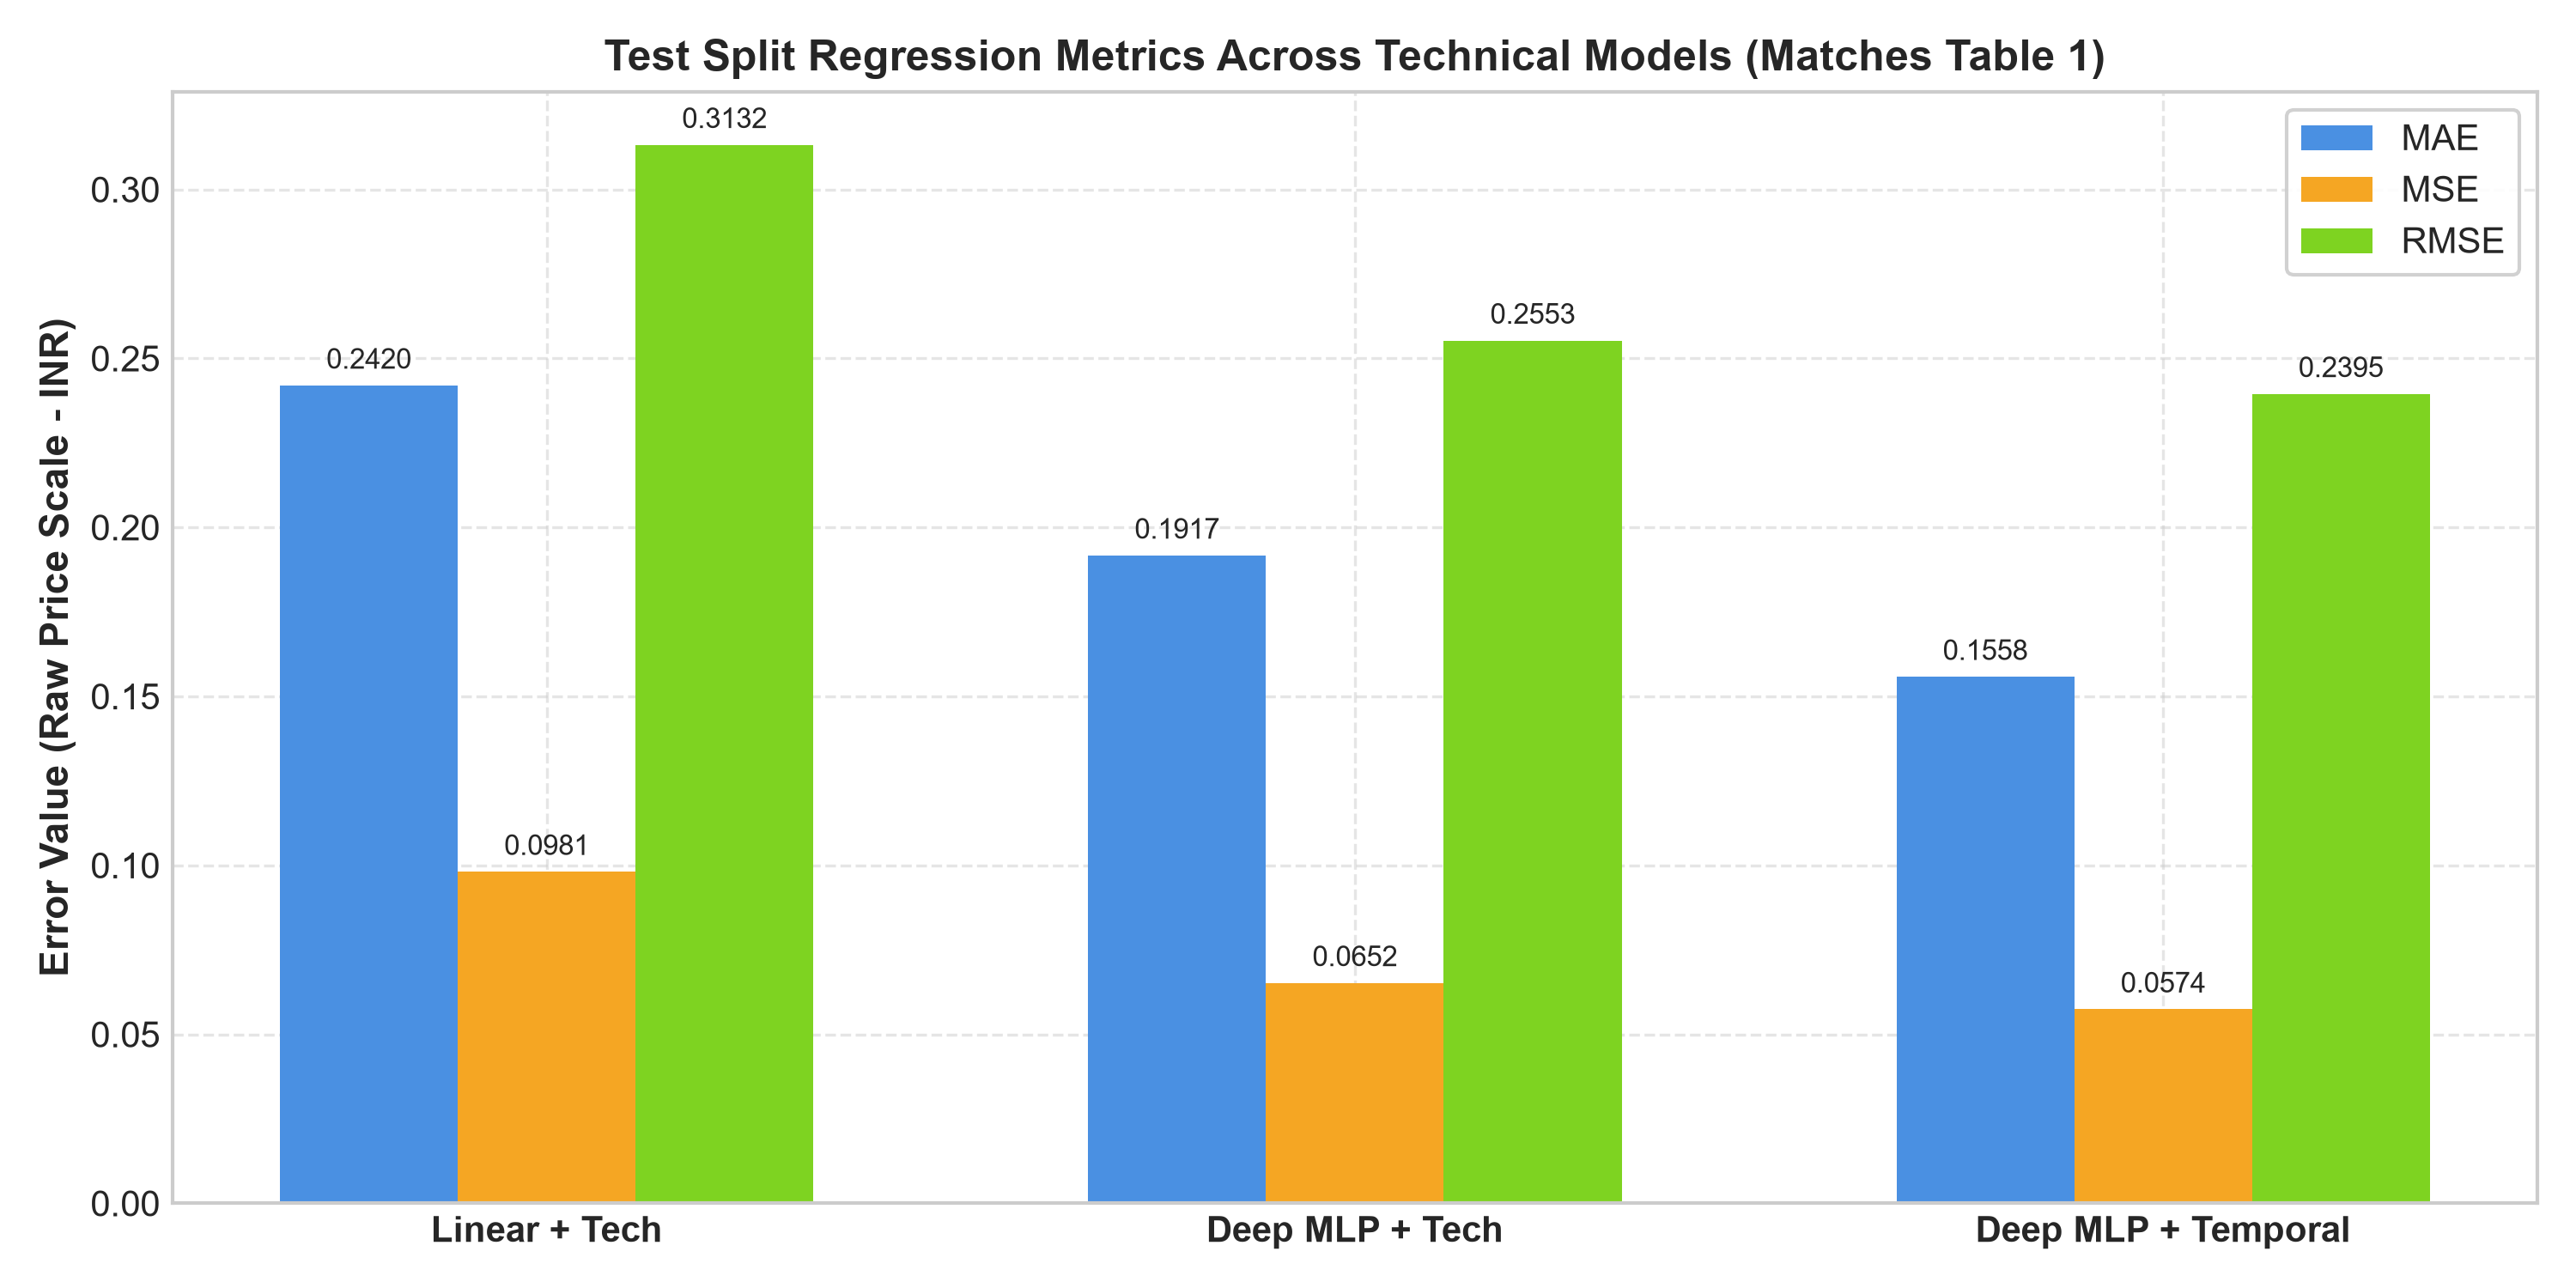
\includegraphics[width=\textwidth]{evaluation-regression-test.png}
\caption{Test-set comparison of MAE, MSE, and RMSE from the evaluation notebook.}
\label{fig:evaluation-regression-test}
\end{figure}

\begin{figure}[htbp]
\centering
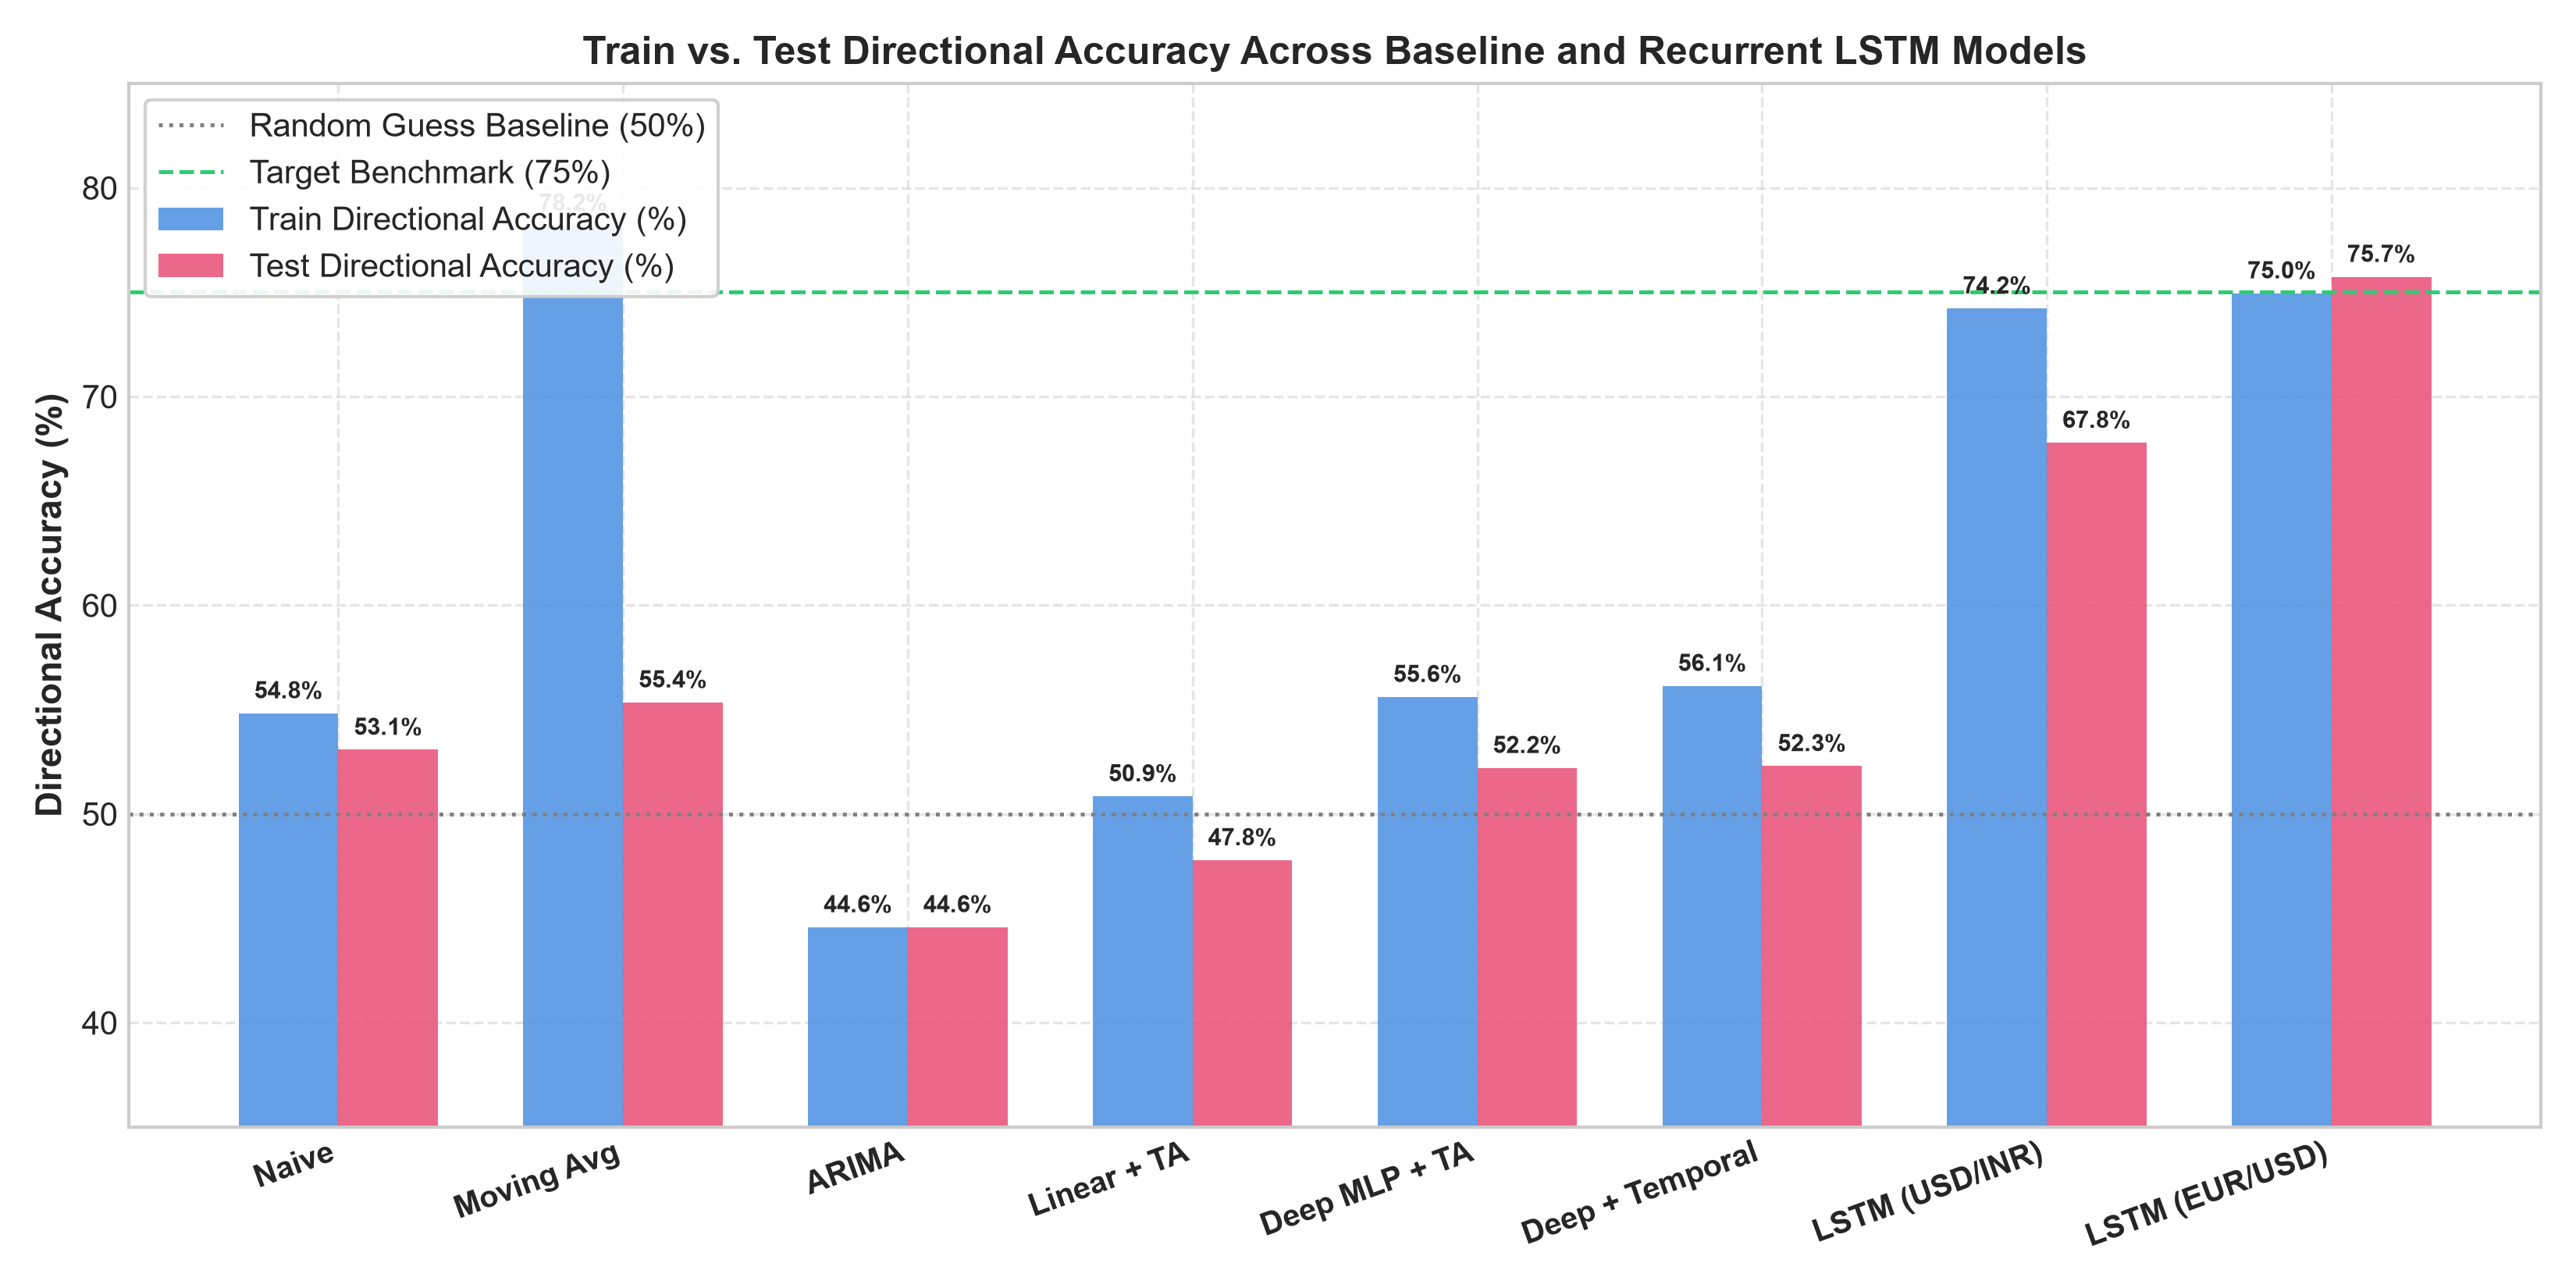
\includegraphics[width=\textwidth]{evaluation-directional-accuracy.png}
\caption{Train and test directional accuracy across the evaluated models.}
\label{fig:evaluation-directional-accuracy}
\end{figure}

\begin{figure}[htbp]
\centering
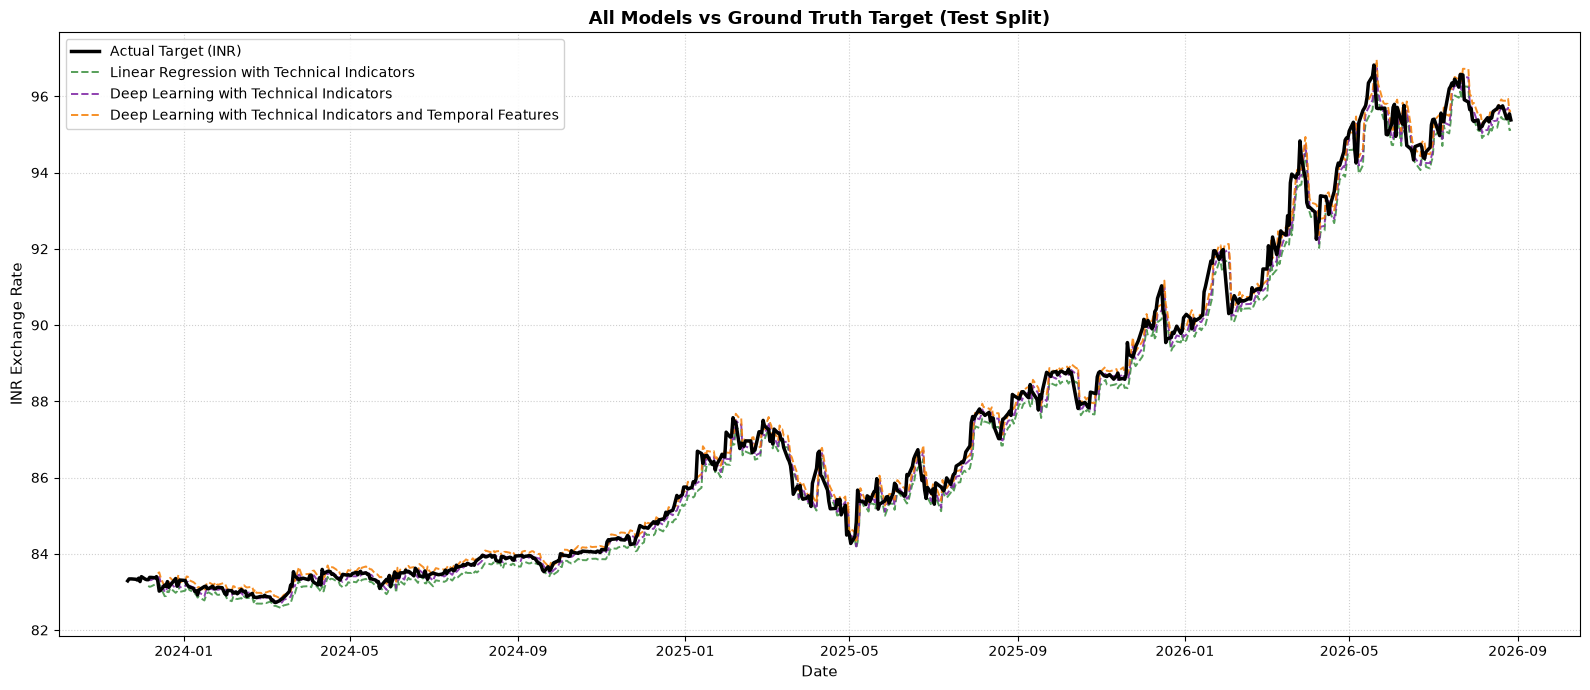
\includegraphics[width=\textwidth]{evaluation-predictions-test.png}
\caption{Held-out test predictions compared with the actual target values.}
\label{fig:evaluation-predictions-test}
\end{figure}

\section{Conclusions and Next Steps}

The literature review indicates that strong reported results depend not only on model capacity but also on the target definition, feature construction, time-series validation, and trading assumptions. The executed experiments provide a transparent comparison between persistence baselines, ARIMA, gradient boosting, linear regression, and fully connected neural networks. The current results also show that technical-indicator preprocessing materially changes the scale and quality of the predictions.

The next steps are to correct the temporal-feature input path, implement and execute the planned LSTM experiment, and add validation metrics for every stored model. Later evaluations should include walk-forward testing, sensitivity to transaction costs, and a clear separation between predictive performance and simulated profitability.

\newpage
\addcontentsline{toc}{section}{References}
\bibliography{document.bib}

\end{document}
